%%%%%%%%%%%%%%%%%%%%%%%%%%%%%%%%%%%%%%%%%%%%%%%%%%%%%%%%%%%%%
%% Begin exercise %%
%%%%%%%%%%%%%%%%%%%%%%%%%%%%%%%%%%%%%%%%%%%%%%%%%%%%%%%%%%%%%
\ex{DC machine and transformer}


\normalsize{\textbf{Acknowledgement}: The following exercise is adapted from ``Grundlagen der Elektrotechnik Teil~B'' by J. Böcker, Paderborn University, 2020}\\



%%%%%%%%%%%%%%%%%%%%%%%%%%%%%%%%%%%%%%%%%%%%%%%%%%%%%%%%%%%%%
%% Task 1 %%
%%%%%%%%%%%%%%%%%%%%%%%%%%%%%%%%%%%%%%%%%%%%%%%%%%%%%%%%%%%%%

\task{Series DC machine with DC and AC voltage supply}
In this task, a ten-pole series DC machine is given. The supply voltage is $U_{\mathrm{DC}}$ = 325 V with an electrical input power of $P_{\mathrm{el}}$ = 500 W at a nominal speed of 1600 $\mathrm{min^{-1}}$.


\subtask{Calculate the nominal torque $\Tn$ and the nominal armature current $I_{\mathrm{a,n}}$ for an effective field inductance of $L_{\mathrm{f}}'$ = 1.24 H.}

\begin{solutionblock}
  The armature current is calculated with:
  \begin{equation}
    I_{\mathrm{a,n}} = \frac{P_{\mathrm{el}}}{U_{\mathrm{DC}}}
    = \frac{\SI{500}{\watt}}{\SI{325}{\volt}}
    = \SI{1.54}{\ampere}.
  \end{equation}

  Hence, the nominal torque calculates as:
  \begin{equation}
    \Tn = L_{\mathrm{f}}' I_{\mathrm{a,n}}^2
    = \SI{1.21}{\henry} \cdot \left(\SI{1.54}{\ampere} \right)^2
    = \SI{2.9}{\newton \metre}.
  \end{equation}
\end{solutionblock}


%%%%%%%%%%%%%%%%%%%%%%%%%%%%%%%%%%%%%%%%%%%%%%%%%%%%%%%%%%%%%
\subtask{Determine the efficiency for the given operating point.}

\begin{solutionblock}
  The mechanical power is given with
  \begin{equation}
    P_{\mathrm{mech}} = \Tn \omega_{\mathrm{n}}
    = \SI{2.9}{\newton \metre} \cdot 2 \pi \cdot \SI{\frac{1600}{60}}
    { \per \second}
    = \SI{486}{\watt}.
  \end{equation}

  The electrical input power is known from the task description, which results in the following efficiency:
  \begin{equation}
    \eta = \frac{P_{\mathrm{mech}}}{P_{\mathrm{el}}}
    = \frac{\SI{486}{\watt}}{\SI{500}{\watt}}
    = 0.972 = \SI{97.2}{\%}.
  \end{equation}
\end{solutionblock}


%%%%%%%%%%%%%%%%%%%%%%%%%%%%%%%%%%%%%%%%%%%%%%%%%%%%%%%%%%%%%
\subtask{The machine is manufactured with a lap winding, which contains $N_{\mathrm{a}}$ = 40 armature windings. The number of field windings $N_{\mathrm{f}}$ = 10 is given too. Calculate the field inductance $L_{\mathrm{f}}$.}

\begin{solutionblock}
  
  The field inductive is calculated with:
  \begin{equation}
    L_{\mathrm{f}} = L_{\mathrm{f}}' \frac{N_{\mathrm{f}}}{N_{\mathrm{a}}} \frac{a \pi}{2p}
    = \SI{1.24}{\henry} \cdot \frac{10}{40} \cdot \frac{5 \pi}{2 \cdot 5}
    = \SI{0.49}{\henry},
  \end{equation}
  where $a=p$ due to the lap winding.
\end{solutionblock}

%%%%%%%%%%%%%%%%%%%%%%%%%%%%%%%%%%%%%%%%%%%%%%%%%%%%%%%%%%%%%
\subtask{Calculate the peak and the average torque of the machine for an alternating voltage supply with $U$~=~230~V and a frequency $f$~=~50~Hz. Assume, that the armature inductivity is given as $L_{\mathrm{a}} = L_{\mathrm{f}} \frac{N_{\mathrm{a}}}{N_{\mathrm{f}}}$.
Interpret the results.}

\begin{solutionblock}
  
  The total series inductance is calculated with:
  \begin{equation}
    L = L_{\mathrm{a}} + L_{\mathrm{f}}
    = L_{\mathrm{f}} \frac{N_{\mathrm{a}}}{N_{\mathrm{f}}} + L_{\mathrm{f}}
    = \SI{0.49}{\henry} \cdot \frac{40}{10} + \SI{0.49}{\henry}
    = \SI{2.43}{\henry}.
  \end{equation}

  The effective resistance can be calculated on the previously provided information from the DC operation case:
  \begin{equation}
    R'(\omega) = \frac{U_{\mathrm{DC}}}{I_{\mathrm{a,n}}}
    = \frac{\SI{325}{\volt}}{\SI{1.54}{\ampere}}
    = \SI{211}{\Omega}.
  \end{equation}

  Therefore, the peak torque is calculated with:
  \begin{equation}
    \hat{T} = 2 L_{\mathrm{f}}' \frac{U^2}{R'(\omega)^2 + \omega_{\mathrm{el}}^2 L^2}
    = 2 \cdot \SI{1.24}{\henry} \cdot \frac{\left(\SI{230}{\volt}\right)^2}{\left(\SI{211}{\Omega}\right)^2 + \left(2\pi \cdot \SI{50}{\hertz}\right)^2 \cdot \left(\SI{2.43}{\henry} \right)^2}
    = \SI{0.21}{\newton \metre}.
  \end{equation}

  The average torque is defined as:
  \begin{equation}
    T = \frac{1}{2} \hat{T}
    = \frac{1}{2} \cdot \SI{0.21}{\newton \metre}
    = \SI{0.11}{\newton \metre}.
  \end{equation}

  The machine in this task is designed for a DC voltage supply, which is shown indirectly with the good efficiency.
  By considering an AC voltage supply, the high inductance value increases the induced voltage significantly. Hence, no voltage margin remains between the terminal voltage and the induced voltage, which results in a small armature current and a small corresponding torque.
  To complete this task: When the series DC machine is designed for a DC voltage supply, the operation with an AC voltage does not make sense but requires an electromagnetic redesign of the machine.

\end{solutionblock}



%%%%%%%%%%%%%%%%%%%%%%%%%%%%%%%%%%%%%%%%%%%%%%%%%%%%%%%%%%%%%
%% Task 2 %%
%%%%%%%%%%%%%%%%%%%%%%%%%%%%%%%%%%%%%%%%%%%%%%%%%%%%%%%%%%%%%

\task{Ideal transformer}
Given is an ideal (no losses, no flux leakage) single-phase transformer with an apparent power of 5 kVA. The voltage $U_{\mathrm{1}}$ on the primary side is 230 V and on the secondary side $U_{\mathrm{2}}$ = 110 V. The transformer is operated at a frequency of 50 Hz.

%%%%%%%%%%%%%%%%%%%%%%%%%%%%%%%%%%%%%%%%%%%%%%%%%%%%%%%%%%%%%
\subtask{Determine the turn ratio $\ddot{u}$ of the transformer.}

\begin{solutionblock}
  The turn ratio of the transformer is given with:
  \begin{equation}
    \ddot{u} = \frac{U_{\mathrm{1}}}{U_{\mathrm{2}}}
    = \frac{\SI{230}{\volt}}{\SI{110}{\volt}}
    = 2.1.
  \end{equation}


\end{solutionblock}


%%%%%%%%%%%%%%%%%%%%%%%%%%%%%%%%%%%%%%%%%%%%%%%%%%%%%%%%%%%%%
\subtask{The transformer is operated at its rated operating point. Calculate the current through the primary and secondary winding.}

\begin{solutionblock}
  The current through the primary winding is calculated as
  \begin{equation}
    I_{\mathrm{1,n}} = \frac{S}{U_{\mathrm{1}}}
    = \frac{\SI{5}{\kilo \watt}}{\SI{230}{\volt}}
    = \SI{21.4}{\ampere},
  \end{equation}
  with the apparent power $S$ given in the task.
  Due to the ideal transformer, the current through the secondary winding is determined in the same way as follows: 
  \begin{equation}
    I_{\mathrm{2,n}} = \frac{S}{U_{\mathrm{2}}}
    = \frac{\SI{5}{\kilo \watt}}{\SI{110}{\volt}}
    = \SI{45.5}{\ampere}.
  \end{equation}

\end{solutionblock}


%%%%%%%%%%%%%%%%%%%%%%%%%%%%%%%%%%%%%%%%%%%%%%%%%%%%%%%%%%%%%
\subtask{Now, the transformer is operated on the secondary side with the rated terminal voltage and delivers an active power of $P_{\mathrm{2}}$ = 3.2 kW with a power factor of $\cos \varphi$ = 0.8 (inductive). Calculate the current of the primary and secondary winding.}

\begin{solutionblock}
  
  The apparent power is calculated with as:
  \begin{equation}
    S = \frac{P_{\mathrm{2}}}{\cos \varphi}
    = \frac{\SI{3.2}{\kilo \watt}}{0.8}
    = \SI{4}{\kilo\volt\ampere}.
  \end{equation}

  Due to the loss-free transformer, the calculated apparent power is the same on the primary and secondary side. Hence, the primary and secondary currents are are determined by:
  \begin{align}
    \begin{split}
      I_{\mathrm{2}} = \frac{S}{U_{\mathrm{2}}}
      = \frac{\SI{4}{\kilo\volt\ampere}}{\SI{110}{\volt}}
      = \SI{36.4}{\ampere}, \\
      I_{\mathrm{1}} = \frac{S}{U_{\mathrm{1}}}
      = \frac{\SI{4}{\kilo\volt\ampere}}{\SI{230}{\volt}}
      = \SI{17.4}{\ampere}.
    \end{split}
  \end{align}
\end{solutionblock}






%%%%%%%%%%%%%%%%%%%%%%%%%%%%%%%%%%%%%%%%%%%%%%%%%%%%%%%%%%%%%
%% Task 3 %%
%%%%%%%%%%%%%%%%%%%%%%%%%%%%%%%%%%%%%%%%%%%%%%%%%%%%%%%%%%%%%

\task{Magnetization current}
A transformer has a primary voltage of $U_{\mathrm{1}}$ = 230 V and a secondary voltage of $U_{\mathrm{2}}$ = 48 V with a frequency of $f$ = 50 Hz. The area of the iron core is $S_{\mathrm{Fe}}$ = $\SI{6}{\centi \metre \squared}$. The average length of the iron core is given with $l_{\mathrm{Fe}}$ = 30 cm. A simplified sketch of the transformer is shown on the left side in Fig.~\ref{fig:transformer_magnetizationCurrent} below. On the right side, the magnetization curve of the utilized iron is visualized.

\begin{figure}[htb]
  \centering
  \includestandalone{ex03/transformer}
  \caption{The left side shows a simplified sketch of the transformer given in the task. On the right hand side a magnetization curve is given.}
  \label{fig:transformer_magnetizationCurrent}
\end{figure}



%%%%%%%%%%%%%%%%%%%%%%%%%%%%%%%%%%%%%%%%%%%%%%%%%%%%%%%%%%%%%
\subtask{How many winding turns are necessary, such that the maximal flux denxity in the iron is $\hat{B}$~=~0.8~T?
Hint: For the calculation of the winding turns, the magnetic coupling of the coils is assumed to be ideal. In addition, winding resistances are also neglected.
Draw the T-equivalent circuit diagram for the given assumptions.}

\begin{solutionblock}
  As described in the task, the windings are perfectly connected, which means, that no leakage flux occurs. In addition, the winding resistances and the iron losses of the transformer are neglected. This results in the equivalent circuit diagram shown in Fig.~\ref{fig:ex_transformer_T_ECD_core_losses_no_load}.
  \begin{solutionfigure}
    \centering
    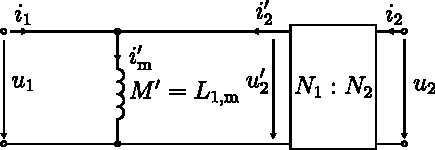
\includegraphics{ex03/ex_transformer_T_ECD_core_losses_no_load.pdf}
    \caption{Equivalent circuit diagram without leakage flux and neglected winding and iron losses.}
    \label{fig:ex_transformer_T_ECD_core_losses_no_load}
  \end{solutionfigure}


  Therefore, the relationship between the voltage and flux linkage is given with:
  \begin{equation}
    u_{\mathrm{1}}(t) = -\frac{\mathrm{d}}{\mathrm{d}t} \psi(t),
  \end{equation}
  which is rearranged into the following form:
  \begin{equation}
    \psi = - \int u_{\mathrm{1}}(t) \mathrm{d}t
    = - \int \sqrt{2} U_{\mathrm{1}} \sin(\omega t) \mathrm{d}t.
  \end{equation}

  Due to the steady state, the integral is indefinite. This results in:
  \begin{equation}
    \psi = \frac{\sqrt{2}U_{\mathrm{1}}}{\omega} \cos(\omega t).
  \end{equation}

  This is simplified in the case of the maximum value of the flux linkage to:
  \begin{equation}
    \hat{\psi} = \frac{\sqrt{2}U_{\mathrm{1}}}{\omega}.
  \end{equation}

  The relationship between the flux linkage, the number of winding turns and flux is given with:
  \begin{equation}
    \psi = N_{\mathrm{1}} \phi_{\mathrm{1}}.
  \end{equation}


  Hence, the number of turns is calculated with:
  \begin{equation}
    N_{\mathrm{1}} = \frac{\hat{\psi}}{\phi}
    = \frac{\frac{\sqrt{2}U_{\mathrm{1}}}{\omega}}{\hat{B} S_{\mathrm{Fe}}}
    =\frac{\frac{\sqrt{2} \cdot \SI{230}{V}}{2\pi \cdot \SI{50}{\hertz}}}{\SI{0.8}{T} \cdot \SI{6\cdot 10^{-4}}{m}}
    = 2157.
    \label{eq:eq1}
  \end{equation}


  The turn ratio of the transformer is defined as follows
  \begin{equation}
    \ddot{u} = \frac{U_{\mathrm{1}}}{U_{\mathrm{2}}}
    = \frac{\SI{230}{\volt}}{\SI{48}{\volt}}
    = 4.79,
  \end{equation}
  hence, the winding turns for the secondary winding are calculated by:
  \begin{equation}
    N_{\mathrm{2}} = \frac{N_{\mathrm{1}}}{\ddot{u}}
    = \frac{2157}{4.79}
    = 451.
  \end{equation}

\end{solutionblock}


%%%%%%%%%%%%%%%%%%%%%%%%%%%%%%%%%%%%%%%%%%%%%%%%%%%%%%%%%%%%%
\subtask{Which magnetization current $I_{\mathrm{m}}'$ consumed the transformer in the no-load operating mode? Assume that the iron losses are neglected.}

\begin{solutionblock}
  
  At no-load operation, the current through the secondary winding is assumed to zero ($i_{\mathrm{2}} = \SI{0}{\ampere}$).
  
  Therefore, the electromotive force simplifies to:
  \begin{equation}
    \theta = H_{\mathrm{Fe}} l_{\mathrm{Fe}}
    = N_{\mathrm{1}} i_{\mathrm{1}}.
  \end{equation}

  Due to the no-load operation, the current through the primary winding is equal to the magnetization current. In addition, the maximum flux density $\hat{B}$ leads to the calculation of the peak magnetization current as:
  \begin{equation}
    \hat{i}_{\mathrm{1}} = \hat{i}_{\mathrm{m,1}}'
    = \frac{\hat{H}_{\mathrm{Fe}} l_{\mathrm{Fe}}}{N_{\mathrm{1}}}
    = \frac{\SI{2}{\ampere \per \centi \metre} \cdot \SI{30}{\centi \metre}}{2157}
    = \SI{27.8}{\milli \ampere}.
  \end{equation}


  The magnetic flux density $B$ shows a linear behavior in the area between 0 T and 0.8 T. Therefore, the magnetization current is not distorted due to the magnetization and has a sinusoidal characteristic.
  Hence, the current is calculated as follows:
  \begin{equation}
    I_{\mathrm{m}}' = \frac{\hat{i}_{\mathrm{m,1}}'}{\sqrt{2}}
    = \frac{\SI{27.8}{\milli\ampere}}{\sqrt{2}}
    = \SI{19.7}{\milli \ampere}.
  \end{equation}

  

\end{solutionblock}


%%%%%%%%%%%%%%%%%%%%%%%%%%%%%%%%%%%%%%%%%%%%%%%%%%%%%%%%%%%%%
\subtask{Calculate the factor between the peak magnetization current $\hat{i}_{\mathrm{m,2}}'$, when the applied voltage is risen from $U_{\mathrm{1}}$ = 230 V to $U_{\mathrm{1}}$ = 400 V.}

\begin{solutionblock}
  With the rearranged equation \eqref{eq:eq1}, the maximum flux density is calculated by:
  \begin{equation}
    \hat{B} = \frac{\sqrt{2} U_{\mathrm{1}}}{\omega S_{\mathrm{Fe}} N_{\mathrm{1}}}
    = \frac{\sqrt{2} \cdot \SI{400}{\volt}}{2\pi \cdot \SI{50}{\hertz} \cdot \SI{6 \cdot 10^{-4}}{\metre} \cdot 2157}
    = \SI{1.39}{\tesla}.
  \end{equation}

  The maximum flux density is used to determine the maximum field strength $\hat{H} = \SI{16}{\ampere \per \centi \metre}$. Hence, the peak magnetization current results in:
  \begin{equation}
    \hat{i}_{\mathrm{m,2}}' = \frac{\hat{H}_{\mathrm{Fe}} l_{\mathrm{Fe}}}{N_{\mathrm{1}}}
    = \frac{\SI{16}{\ampere \per \centi \metre} \cdot \SI{30}{\centi \metre}}{2157}
    = \SI{222.5}{\milli\ampere}.
  \end{equation}

  Hence, the factor is calculated as:
  \begin{equation}
    \frac{\hat{i}_{\mathrm{m,2}}}{\hat{i}_{\mathrm{m,1}}} = \frac{\SI{222.5}{\milli\ampere}}{\SI{27.8}{\milli\ampere}}
    = 8.
  \end{equation}
\end{solutionblock}



%%%%%%%%%%%%%%%%%%%%%%%%%%%%%%%%%%%%%%%%%%%%%%%%%%%%%%%%%%%%%
%% Task 4 %%
%%%%%%%%%%%%%%%%%%%%%%%%%%%%%%%%%%%%%%%%%%%%%%%%%%%%%%%%%%%%%

\task{Parameter identification via no-load test}
Given is a 50 Hz, 6 MVA single-phase transformer with $U_{\mathrm{1}}$ = 5 kV and $U_{\mathrm{2}}$ = 100 kV.
The effective area of the core is $S_{\mathrm{Fe}}$ = 0.187 $\mathrm{m}^2$ and a maximum flux density of $\hat{B}$ = 1.5 T. During the no-load operation, the primary voltage is $U_{\mathrm{1,o}}$ = 5 kV with a no-load electrical power $P_{\mathrm{o}}$ = 8.8 kW and the no-load current $I_{\mathrm{o}}$ = 2.6 A.



%%%%%%%%%%%%%%%%%%%%%%%%%%%%%%%%%%%%%%%%%%%%%%%%%%%%%%%%%%%%%
\subtask{Calculate the nominal currents and the transformer ratio.}

\begin{solutionblock}
  The transformer ratio is given as:
  \begin{equation}
    \ddot{u} = \frac{U_{\mathrm{1}}}{U_{\mathrm{2}}}
    = \frac{\SI{5}{\kilo \volt}}{\SI{100}{\kilo \volt}}
    = 0.05.
  \end{equation}

  With the apparent power $S$ of the transformer, the primary and secondary currents are calculated by:
  \begin{align}
    \begin{split}
      I_{\mathrm{1}} &= \frac{S}{U_{\mathrm{1}}}
      = \frac{\SI{6}{\mega \volt \ampere}}{\SI{5}{\kilo \volt}}
      = \SI{1200}{\ampere}, \\
      I_{\mathrm{2}} &= \frac{S}{U_{\mathrm{2}}}
      = \frac{\SI{6}{\mega \volt \ampere}}{\SI{100}{\kilo \volt}}
      = \SI{60}{\ampere}. \\
    \end{split}
  \end{align}

\end{solutionblock}



%%%%%%%%%%%%%%%%%%%%%%%%%%%%%%%%%%%%%%%%%%%%%%%%%%%%%%%%%%%%%
\subtask{Calculate the number of winding turns $N_{\mathrm{1}}$ for the primary and $N_{\mathrm{2}}$ for the secondary side.}

\begin{solutionblock}
  
  The number of winding turns for the primary side is calculated with:
  \begin{equation}
    N_{\mathrm{1}} = \frac{\hat{\psi}}{\phi}
    = \frac{\frac{\sqrt{2}U_{\mathrm{1}}}{\omega}}{\hat{B} S_{\mathrm{Fe}}}
    = \frac{\frac{\sqrt{2} \cdot \SI{5}{\kilo\volt}}{2\pi \cdot \SI{50}{\hertz}}}{\SI{1.5}{\tesla} \cdot \SI{0.187}{\metre^2}}
    = 81.
    \end{equation}

    The number of winding turns for the secondary side is calculated with the transformer ratio as follows:
    \begin{equation}
      N_{\mathrm{2}} = \frac{N_{\mathrm{1}}}{\ddot{u}}
      = \frac{81}{0.05}
      = 1620.
    \end{equation}
\end{solutionblock}

%%%%%%%%%%%%%%%%%%%%%%%%%%%%%%%%%%%%%%%%%%%%%%%%%%%%%%%%%%%%%
\subtask{Determine the iron losses and the apparent power $S_{\mathrm{o}}$ for no-load operation. Give the values for the magnetization current $I_{\mathrm{m}}'$, the iron loss current $I_{\mathrm{c}}$ and the mutual inductance $M'$. Assume for the calculation that $R_{\mathrm{1}} << R_{\mathrm{c}}$ and $L_{\mathrm{1,\sigma}} << M'$. In addition, draw the equivalent circuit diagram with the given assumptions.}


\begin{solutionblock}

  The equivalent circuit diagram for the no-load operation with the iron loss resistance $R_{\mathrm{c}}$ is shown in Fig.~\ref{fig:ex_transformer_open_circuit_test}.
  \begin{solutionfigure}
    \centering
    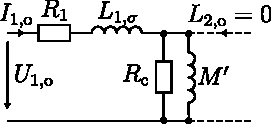
\includegraphics{ex03/ex_Transformer_open_circuit_test.pdf}
    \captionsetup{labelfont={color=blue},textfont={color=blue}}
    \caption{Equivalent circuit diagram for the no-load test with the iron loss resistor $R_{\mathrm{c}}$.}
    \label{fig:ex_transformer_open_circuit_test}
  \end{solutionfigure}
  
  
  The no-load apparent power is calculated by
  \begin{equation}
    S_{\mathrm{o}} = U_{\mathrm{o}} I_{\mathrm{o}}
    = \SI{5}{\kilo\volt} \cdot \SI{2.6}{\ampere}
    = \SI{13}{\kilo\volt\ampere},
  \end{equation}
  with the no-load voltage $U_{\mathrm{o}}$ and the no-load current $I_{\mathrm{o}}$.

  The equivalent iron loss resistance is determine as follows
  \begin{equation}
    R_{\mathrm{c}} = \frac{U_{\mathrm{1,o}}^2}{P_{\mathrm{1,o}}}
    = \frac{\left(\SI{5}{\kilo\volt} \right)^2}{\SI{8.8}{\kilo\watt}}
    = \SI{2841}{\Omega},
  \end{equation}
  and, therefore, the corresponding current is calculated with:
  \begin{equation}
    I_{\mathrm{c}} = \sqrt{\frac{P_{\mathrm{1,o}}}{R_{\mathrm{c}}}}
    = \sqrt{\frac{\SI{8.8}{\kilo\watt}}{\SI{2841}{\Omega}}}
    = \SI{1.76}{\ampere}.
  \end{equation}

  The power factor is determined as
  \begin{equation}
    \cos \varphi_{\mathrm{o}} = \frac{P}{S}
    = \frac{\SI{8.8}{\kilo\watt}}{\SI{13}{\kilo\volt\ampere}}
    = 0.68,
  \end{equation}
  and the corresponding angle is $\varphi_{\mathrm{o}} = \SI{47.16}{\degree}$.

  The following equation is used to calculate the mutual inductance
  \begin{equation}
    \omega_{\mathrm{el}} M' \approx \frac{U_{\mathrm{1,o}}}{I_{\mathrm{1,o}} \sin(\varphi_{\mathrm{o}})},
  \end{equation}
  which is rearranged to:
  \begin{equation}
    M' = \frac{U_{\mathrm{1,o}}}{I_{\mathrm{1,o}} \sin(\varphi_{\mathrm{o}}) \omega_{\mathrm{el}}}
    = \frac{\SI{5}{\kilo\volt}}{\SI{2.6}{\ampere}\cdot \sin(\SI{47.16}{\degree})\cdot 2\pi \cdot \SI{50}{\hertz}}
    = \SI{8.35}{\henry}.
  \end{equation}

  With the geometric addition the magnetization currents is calculated with:
  \begin{equation}
    I_{\mathrm{m}}' = \sqrt{I_{\mathrm{1,o}}^2 - I_{\mathrm{c}}^2}
    = \sqrt{\left(\SI{2.6}{\ampere} \right)^2 - \left(\SI{1.76}{\ampere}\right)^2}
    = \SI{1.91}{\ampere}.
  \end{equation}

\end{solutionblock}







%%%%%%%%%%%%%%%%%%%%%%%%%%%%%%%%%%%%%%%%%%%%%%%%%%%%%%%%%%%%%
%% Task 5 %%
%%%%%%%%%%%%%%%%%%%%%%%%%%%%%%%%%%%%%%%%%%%%%%%%%%%%%%%%%%%%%

\task{Inrush current}
Given is a single-phase transformer in no-load operation (i.e., open circuit secondary side) which initial primary current is zero. A the time point $t$ = 0, the voltage $u_{\mathrm{n}}(t) = \hat{u}_{\mathrm{n}} \sin (\omega t + \alpha)$ is applied.
Remanence and iron losses are neglected.
The self-inductance $L_{\mathrm{1}}$, resistance $R_{\mathrm{1}}$ and the number of winding turns $N_{\mathrm{1}}$ are given.

%%%%%%%%%%%%%%%%%%%%%%%%%%%%%%%%%%%%%%%%%%%%%%%%%%%%%%%%%%%%%
\subtask{Calculate the inrush current trajectory $i_{\mathrm{1}}(t)$ and the trajectory of the flux $\phi (t)$.}

\begin{solutionblock}
  
  The dynamic equation of the transformer current is given as follows:
  \begin{equation}
    \frac{\mathrm{d}}{\mathrm{d}t}\bm{i}(t) = \begin{bmatrix} -\frac{R_1}{\sigma L_1} & \frac{R_2 M}{\sigma L_1 L_2} \\ \frac{R_1 M}{\sigma L_1 L_2} & -\frac{R_2}{\sigma L_2} \end{bmatrix} \bm{i}(t) + \begin{bmatrix} \frac{1}{\sigma L_1} & -\frac{M}{\sigma L_1 L_2} \\ -\frac{M}{\sigma L_1 L_2} & \frac{1}{\sigma L_2} \end{bmatrix} \bm{u}(t).
  \end{equation}

  Due to the no-load operation ($i_{\mathrm{2}} = \SI{0}{\ampere}$) and the neglected leakage flux, the equation simplifies to:
  \begin{equation}
    \frac{\mathrm{d}}{\mathrm{d}t} i_{\mathrm{1}}(t) = -\frac{R_{\mathrm{1}}}{L_{\mathrm{1}}}i_{\mathrm{1}}(t) -\frac{1}{L_{\mathrm{1}}} u_{\mathrm{1}}(t).
  \end{equation}

  The equation from above is rearranged to solve the ordinary differential equation. Therefore, the homogeneous part is on the left side and the perturbation part on the right side as given below
  \begin{equation}
    \frac{\mathrm{d}}{\mathrm{d}t} i_{\mathrm{1}}(t) + \frac{1}{\tau} i_{\mathrm{1}}(t) = \frac{1}{L_{\mathrm{1}}} u_{\mathrm{1}}(t),
    \label{eq:ode}
  \end{equation}
  with $\tau = \frac{L_{\mathrm{1}}}{R_{\mathrm{1}}}$.
  
  First, the homogeneous part is separated, which results in:
  \begin{equation}
    \frac{\mathrm{d}}{\mathrm{d}t} i_{\mathrm{1}}(t) + \frac{1}{\tau} i_{\mathrm{1}}(t) = 0.
  \end{equation}

  This homogeneous part is solved with the exponential approach, which is given with
  \begin{equation}
    i_{\mathrm{1}}(t) = C e^{-\frac{t}{\tau}},
    \label{eq:ode_approach_hom}
  \end{equation}
  and the first derivative
  \begin{equation}
    \frac{\mathrm{d}}{\mathrm{d}t}i_{\mathrm{1}}(t) = -\frac{C}{\tau} e^{-\frac{t}{\tau}},
    \label{eq:ode_approach_hom_derivative}
  \end{equation}
  with an integration constant $C$.

  Using \eqref{eq:ode_approach_hom} and \eqref{eq:ode_approach_hom_derivative} results in
  \begin{equation}
    \frac{R_{\mathrm{1}}}{L_{\mathrm{1}}} C e^{-\frac{t}{\tau}} - \frac{C}{\tau} e^{-\frac{t}{\tau}} = 0,
  \end{equation}
  which is rearranged as follows:
  \begin{equation}
    C e^{-\frac{t}{\tau}} \left(\frac{R_{\mathrm{1}}}{L_{\mathrm{1}}}-\frac{t}{\tau} \right)=0.
  \end{equation}


  Therefore, the homogeneous solution is given as:
  \begin{equation}
    i_{\mathrm{1,h}}(t) = C e^{-\frac{t}{\tau}}.
  \end{equation}
  

  In the second step, the perturbation solution is determined. Therefore, the comparison of coefficients ansatz is used.
  The voltage is given in the task with
  \begin{equation}
    u_{\mathrm{n}} = \hat{u}_{\mathrm{n}} \sin(\omega t + \alpha),
  \end{equation}
  which leads to:
  \begin{equation}
    \sin(\omega t + \alpha) = \cos(\omega t) \sin(\alpha) + \sin(\omega t) \cos(\alpha).
    \label{eq:ode_perturbation}
  \end{equation}

  The expression in \eqref{eq:ode_perturbation} is separated in two parts which are later combined again (superposition principle of linear systems). The approach for the first case is given by:
  \begin{equation}
    \frac{\mathrm{d}}{\mathrm{d}t}i(t) + \frac{1}{\tau}i(t) = k \sin(\alpha) \cos(\omega t),
  \end{equation}
  with a new parameter $k = \frac{\hat{u}}{L_{\mathrm{1}}}$, derived from \eqref{eq:ode}.

  The general approach is given with
  \begin{equation}
    i_{\mathrm{1,s}}(t) = a \cos(\omega t) + b \sin(\omega t),
    \label{eq:ode_approach_per}
  \end{equation}
  with the two parameter $a$ and $b$. The first derivative is determined as:
  \begin{equation}
    \frac{\mathrm{d}}{\mathrm{d}t} i_{\mathrm{1,s}}(t) = - a \omega \sin(\omega t) + b \omega \cos(\omega t).
    \label{eq:ode_approach_per_derivative}
  \end{equation}

  With \eqref{eq:ode_approach_per} and \eqref{eq:ode_approach_per_derivative} in \eqref{eq:ode} the equation is determined:
  \begin{equation}
    - a \omega \sin(\omega t) + b \omega \cos(\omega t) + \frac{1}{\tau} \left[a \cos(\omega t) + b \sin(\omega t)  \right]
    = k \sin(\alpha) \cos(\omega t).
  \end{equation}

  The following equation is obtained by reshaping
  \begin{equation}
    \sin(\omega t) \left[-a \omega + \frac{1}{\tau} b \right] + \cos(\omega t) \left[b\omega + \frac{1}{\tau} a - k \sin(\omega t) \right] = 0,
  \end{equation}
  and by dividing through $\cos(\omega t)$ results in:
  \begin{equation}
    \tan(\omega t) \left[-a \omega + \frac{1}{\tau} b \right] + \left[b \omega + \frac{1}{\tau}a - k \sin(\omega t) \right] = 0.
  \end{equation}

  To fulfill the equation, the expressions between the large brackets must be zero. 
  The first expression is given with:
  \begin{align}
    \begin{split}
      -a\omega + &\frac{1}{\tau}b = 0, \\
      b &= a \omega \tau.
      \label{eq:ode_b}
    \end{split}
  \end{align}

  The second expression is defined with:
  \begin{equation}
    b \omega + \frac{1}{\tau} a - k \sin(\alpha) = 0.
  \end{equation}

  With $b$ from \eqref{eq:ode_b} results in
  \begin{align}
    \begin{split}
      a \omega^2 \tau + \frac{1}{\tau} a - k \sin(\alpha) = 0, \\
      a \left[\omega^2 \tau + \frac{1}{\tau} \right] = k \sin(\alpha),
    \end{split}
  \end{align}

  which is reshaped to:
  \begin{equation}
    a = \frac{k \sin(\alpha)}{\omega^2 \tau + \frac{1}{\tau}}.
  \end{equation}

  Therefore, with the two calculated coefficients, the solution for the first approach is: 
  \begin{equation}
    i_{\mathrm{1,s}}(t) = \frac{k \sin(\alpha)}{\omega^2 \tau + \frac{1}{\tau}} \left[\cos(\omega t) + \omega \tau \sin(\omega t) \right].
  \end{equation}


  The second case is given with $\frac{\mathrm{d}}{\mathrm{d}t}i(t) + \frac{1}{\tau}i(t) = k \cos(\alpha) \sin(\omega t)$.To do this, the steps already carried out in the first approach are repeated.
  The starting point is given as
  \begin{equation}
    i_{\mathrm{2,s}}(t) = a \cos(\omega t) + b \sin(\omega t),
  \end{equation}
  and, therefore, the first derivative:
  \begin{equation}
    \frac{\mathrm{d}}{\mathrm{d}t} i_{\mathrm{2,s}}(t) = - a \omega \sin(\omega t) + b \omega \cos(\omega t).
  \end{equation}

  The comparison of coefficients and reshaping leads to:
  \begin{align}
    \begin{split}
    -a \omega \sin(\omega t) + b \omega \cos(\omega t) = \frac{1}{\tau} \left[a \cos(\omega t) + b\sin(\omega t) \right] &= k \sin(\omega t), \\
    \sin(\omega t) \left[-a \omega + \frac{1}{\tau}b - k\cos(\alpha)\right] + \cos(\omega t) \left[b \omega + \frac{1}{\tau}a \right] &= 0.
    \end{split}
  \end{align}

  To fulfill the equation, the expressions between the large brackets must be zero. 
  The first expression is given with:
  \begin{align}
    \begin{split}
      b \omega + &\frac{1}{\tau}a =0, \\
      a &= \omega b \tau.
      \label{eq:ode_parameter_a}
    \end{split}
  \end{align}

  The second expression is defined with:
  \begin{align}
    \begin{split}
      -a \omega + &\frac{1}{\tau}b - k\cos(\alpha) = 0, \\
      \omega^2 b \tau + &\frac{1}{\tau}b - k \cos(\alpha) = 0, \\
      b &= \frac{k\cos(\alpha)}{\omega^2\tau+\frac{1}{\tau}}.
    \end{split}
  \end{align}

  This result is used to solve parameter $a$ from \eqref{eq:ode_parameter_a} as follows:
  \begin{equation}
    a = -\omega b \tau = -\frac{\omega \tau k \cos(\alpha)}{\omega^2\tau + \frac{1}{\tau}}.
  \end{equation}

  Therefore, the solution for the second case of the perturbation part is defined as
  \begin{equation}
    i_{\mathrm{s,2}}(t) = \frac{k\cos(\alpha)}{\omega^2 \tau + \frac{1}{\tau}} \left[-\omega \tau \cos(\omega t) + \sin(\omega t) \right],
    \end{equation}

 and, this leads to the solution of the perturbation part by:
  \begin{equation}
    i_{\mathrm{1,s}}(t) = \frac{k}{\omega^2 \tau + \frac{1}{\tau}}
    \left[
      \sin(\alpha)\left[\cos(\omega t) + \omega \tau \sin(\omega t) \right]
      + \cos(\alpha) \left[-\omega \tau \cos(\omega t) + \sin(\omega t) \right]
    \right].
  \end{equation}

  The total solution is given with:
  \begin{equation}
    i_{\mathrm{1}}(t) = i_{\mathrm{1,h}}(t) + i_{\mathrm{1,s}}(t).
  \end{equation}


  Next, the integration constant $C$ from the homogeneous solution is determined. To perform this, the initial conditions are used, which are defined in the task description. Therefore, the current is defined as:
  \begin{equation}
    i_{\mathrm{1}}(0) = 0.
    \label{eq:ode_initialCondition}
  \end{equation}
  
  The second initial condition is the results of applying \eqref{eq:ode_initialCondition} to the differential equation, that is:
  \begin{equation}
    \frac{\mathrm{d}}{\mathrm{d}t}i_{\mathrm{1}}(0) = \frac{1}{L_{\mathrm{1}}}u(0) = \frac{1}{L_{\mathrm{1}}} \hat{u}\sin(\alpha).
  \end{equation}

  Apply the initial conditions to the total solution results in
  \begin{equation}
    i(0) = C + \frac{k}{\omega^2 \tau + \frac{1}{\tau}}
    \left[\sin(\alpha) - \omega \tau \cos(\alpha) \right] = 0,
  \end{equation}
  which is rearranged to:
  \begin{equation}
    C = \frac{k}{\omega^2\tau + \frac{1}{\tau}} \left[-\sin(\alpha) + \omega \tau \cos(\alpha) \right].
  \end{equation}

  Therefore, the total solution is given with:
  \begin{align}
    \begin{split}
      i_{\mathrm{1}}(t) &=\frac{k}{\omega^2\tau + \frac{1}{\tau}} \left[-\sin(\alpha) + \omega \tau \cos(\alpha) \right] e^{-\frac{t}{\tau}} \\
      &+\frac{k}{\omega^2 \tau + \frac{1}{\tau}}
      \left[
        \sin(\alpha)\left[\cos(\omega t) + \omega \tau \sin(\omega t) \right]
        + \cos(\alpha) \left[-\omega \tau \cos(\omega t) + \sin(\omega t) \right]
      \right].
      \label{eq:ode_solution}
  \end{split}
  \end{align}

  The trajectory of the flux is defined as
  \begin{equation}
    \phi(t) = L_{\mathrm{1}} i(t),
  \end{equation}
  and, therefore, directly given with the current trajectory.
\end{solutionblock}



%%%%%%%%%%%%%%%%%%%%%%%%%%%%%%%%%%%%%%%%%%%%%%%%%%%%%%%%%%%%%
\subtask{Assume that $R_{\mathrm{1}} << \omega L_{\mathrm{1}}$.
Discuss the result for $i_{\mathrm{1}}(t)$, when the voltage is applied at zero crossing with an angle $\alpha$ = 0 and for an angle of $\alpha = \frac{\pi}{2}$.}

\begin{solutionblock}

  First, the trajectory for $\alpha$ = 0 is determined. Therefore, \eqref{eq:ode_solution} results in:
  \begin{equation}
    i_{\mathrm{1}}(t) = \frac{k}{\omega^2\tau+\frac{1}{\tau}} \left[\omega \tau e^{-\frac{t}{\tau}} - \omega \tau \cos(\omega t) + \sin(\omega t) \right].
  \end{equation}

  With the assumptions given in the task, $R_{\mathrm{1}} << L_{\mathrm{1}} \omega$
  results into $\omega \tau >> 1$.

  Hence, the equation simplifies to
  \begin{align}
    \begin{split}
      i_{\mathrm{1}}(t) &= \frac{k}{\omega^2\tau + \frac{1}{\tau}} \omega t \left[e^{-\frac{t}{\tau}} - \cos(\omega t) \right], \\
      &= \frac{\hat{u}}{L_{\mathrm{1}}} \frac{1}{\omega} \left[e^{-\frac{t}{\tau}} - \cos(\omega t) \right],
    \end{split}
  \end{align}
  which is used to calculate the current trajectory. 
  As it can be seen, the equation contains an exponential part. To determine the steady-state current trajectory, the equation is reshaped into:
  \begin{align}
    \begin{split}
    i_{\mathrm{1}}(t) = \frac{\hat{u}}{L_{\mathrm{1}}\omega}e^{-\frac{t}{\tau}}-\frac{\hat{u}}{L_{\mathrm{1}}\omega}\cos(\omega t), \\
    = \frac{\hat{u}}{L_{\mathrm{1}}\omega}e^{-\frac{t}{\tau}} + \frac{\hat{u}}{L_{\mathrm{1}}} \int \sin(\omega t) \mathrm{d}t.
    \end{split}
  \end{align}

  With the input voltage $u(t) = \hat{u}\sin(\omega t + \alpha)$, the equation simplifies to:
  \begin{equation}
    i_{\mathrm{1}}(t) = \frac{\hat{U}}{L_{\mathrm{1}}\omega}e^{-\frac{t}{\tau}} + \frac{1}{L_{\mathrm{1}}} \int u(t) \mathrm{d}t.
  \end{equation}

  Assumed, that in the steady state $\tau \rightarrow \infty$, only the second part of the equation remains. Therefore, the current trajectory is given with:
  \begin{equation}
    i_{\mathrm{1}}(t) = \frac{1}{L_{\mathrm{1}}} \int u(t) \mathrm{d}t.
  \end{equation}

  Next, the trajectory for $\alpha = \frac{\pi}{2}$ is determined. Therefore, the equation \eqref{eq:ode_solution} is solved as follows:
  \begin{align}
    \begin{split}
      i_{\mathrm{1}}(t) &= \frac{k}{\omega^2\tau + \frac{1}{\tau}}
      \left[\cos(\omega t) + \omega \tau \sin(\omega t) \right], \\
      &= \frac{k}{\omega^2\tau + \frac{1}{\tau}} \left[\omega \tau \sin(\omega t) \right], \\
      &= \frac{1}{L_{\mathrm{1}}} \hat{U} \frac{1}{\omega} \sin(\omega t), \\
      &= \frac{\hat{U}}{L_{\mathrm{1}}\omega} \sin(\omega t).
    \end{split}
  \end{align}


  In Fig.~\ref{fig:current_transformer} the two calculated current trajectories are visualized. They result from the applied voltage with the additional angle $\alpha$.
  In this example is the peak current value during the transient process approximately double than in the steady state, which can trigger the overcurrent protection. Therefore, the magnetization current should be kept low and the overcurrent protection must be able to handle the inrush current.
  \begin{solutionfigure}
    \centering
    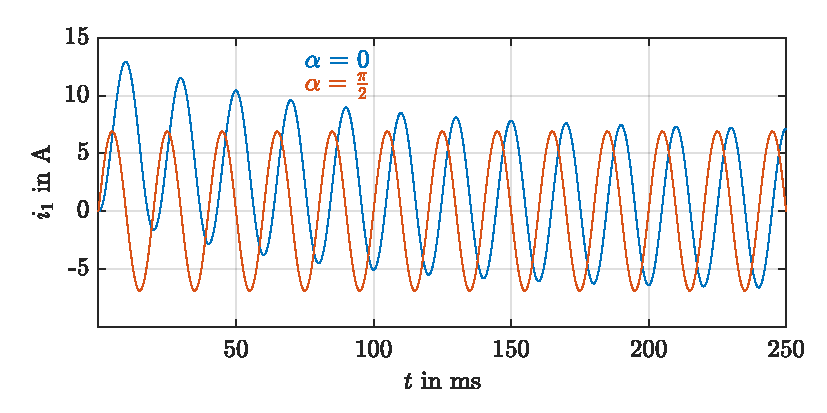
\includegraphics{ex03/current_transformer.pdf}
    \caption{Current of the transformer, when the voltage is applied at two different angles for $\alpha$.}
    \label{fig:current_transformer}
  \end{solutionfigure}
  

\end{solutionblock}